\documentclass[tikz, border=15pt]{standalone}
\usepackage{amsmath, amssymb}
\usepackage{xcolor}
\usepackage{tikz}
\usetikzlibrary{shapes.geometric, arrows.meta, positioning, calc, fit, backgrounds, shadows}

\begin{document}
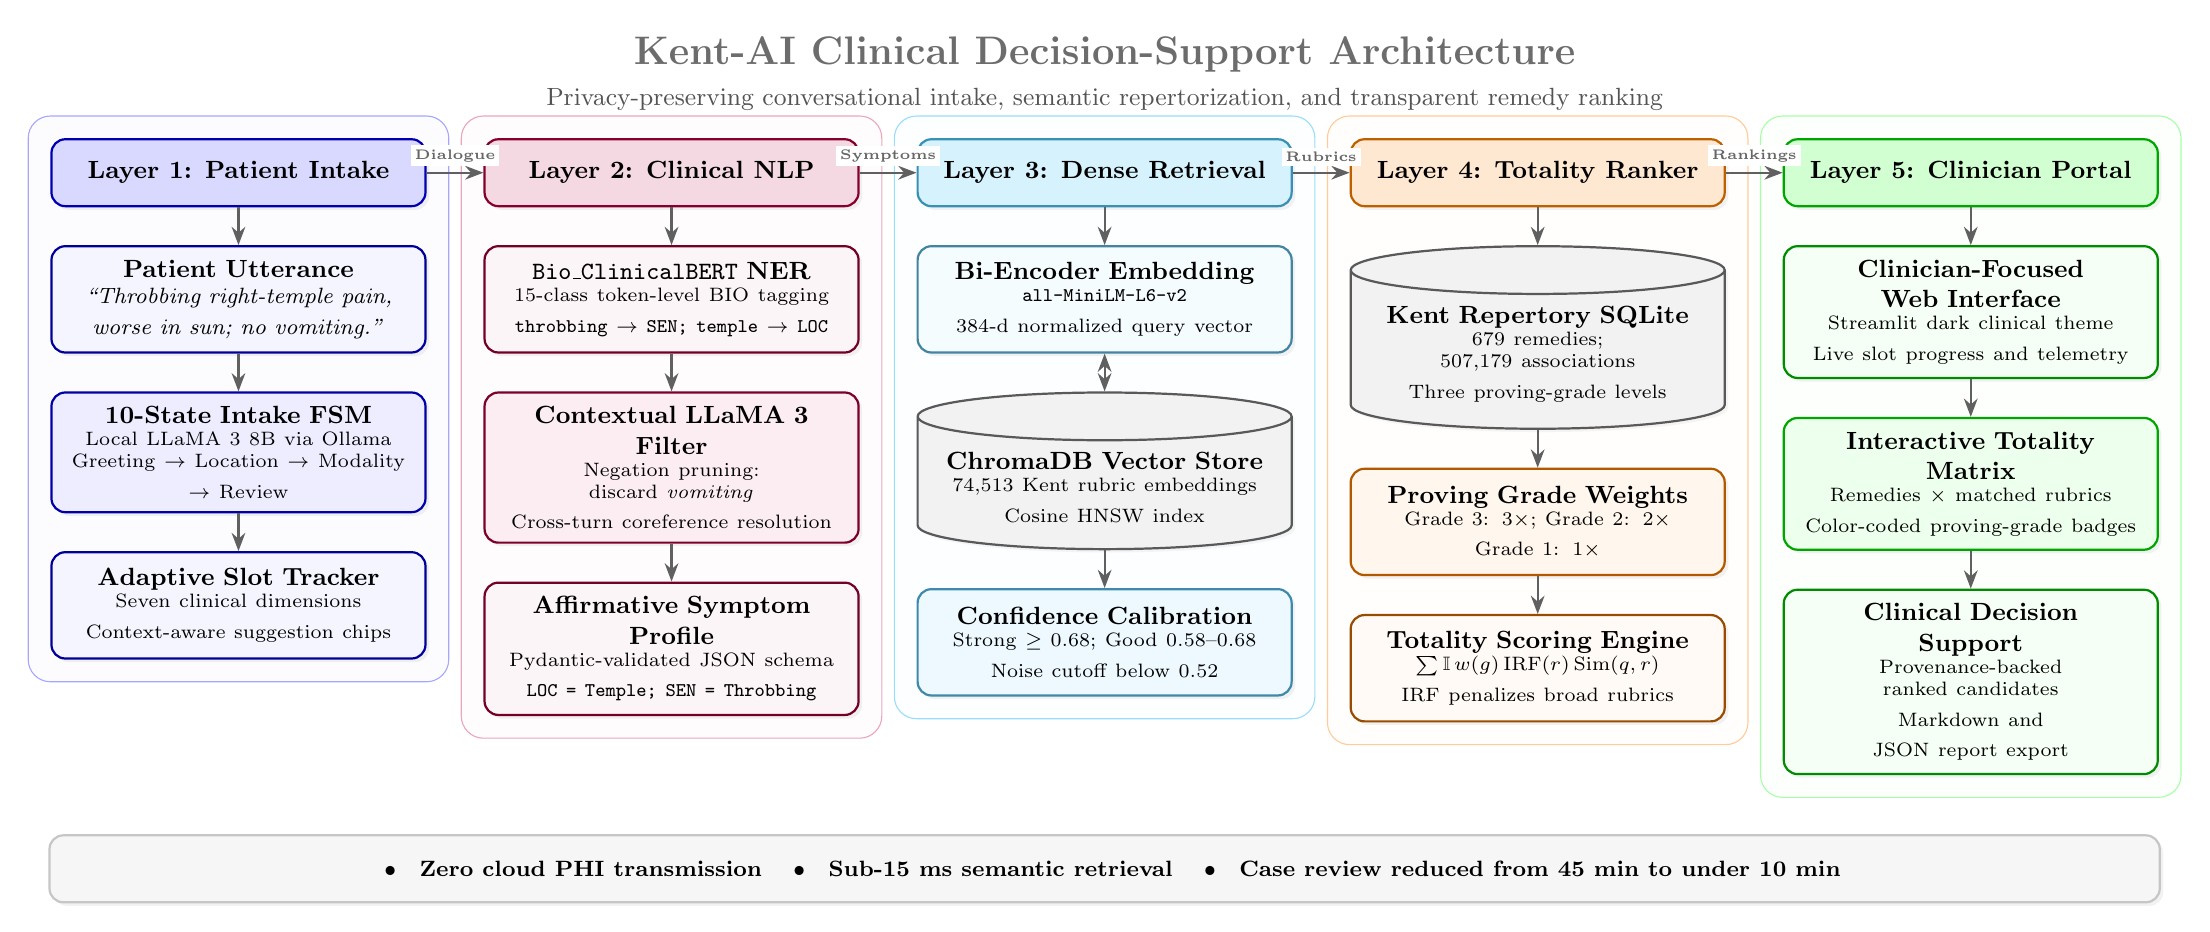
\begin{tikzpicture}[
    font=\sffamily,
    >=Stealth,
    basebox/.style={
        draw,
        rounded corners=5pt,
        align=center,
        thick,
        drop shadow={opacity=0.10, shadow xshift=1.3pt, shadow yshift=-1.3pt}
    },
    colheader/.style={
        basebox,
        minimum width=4.75cm,
        minimum height=0.85cm,
        font=\bfseries\small,
        inner sep=4pt
    },
    subcard/.style={
        basebox,
        minimum width=4.75cm,
        minimum height=1.35cm,
        text width=4.25cm,
        font=\small,
        inner sep=5pt
    },
    dbnode/.style={
        draw,
        cylinder,
        shape border rotate=90,
        aspect=0.14,
        align=center,
        thick,
        fill=gray!10,
        draw=gray!70!black,
        minimum width=4.75cm,
        minimum height=1.35cm,
        text width=4.05cm,
        font=\small,
        inner sep=4pt,
        drop shadow={opacity=0.08, shadow xshift=1.2pt, shadow yshift=-1.2pt}
    },
    arrow/.style={->, thick, draw=gray!75!black},
    darrow/.style={<->, thick, draw=gray!75!black},
    flowlabel/.style={fill=white, font=\tiny\bfseries, inner sep=1.5pt, text=gray!80!black},
    footer/.style={basebox, fill=gray!7, draw=gray!45, minimum width=26.8cm, minimum height=0.85cm, font=\footnotesize}
]

    % Title
    \node[font=\bfseries\Large, text=gray!85!black] at (11,-0.15)
        {Kent-AI Clinical Decision-Support Architecture};
    \node[font=\small, text=gray!65!black] at (11,-0.72)
        {Privacy-preserving conversational intake, semantic repertorization, and transparent remedy ranking};

    % Layer headers
    \node[colheader, fill=blue!15, draw=blue!70!black] at (0,-1.65) (h1) {Layer 1: Patient Intake};
    \node[colheader, fill=purple!15, draw=purple!70!black] at (5.5,-1.65) (h2) {Layer 2: Clinical NLP};
    \node[colheader, fill=cyan!16, draw=cyan!70!black] at (11,-1.65) (h3) {Layer 3: Dense Retrieval};
    \node[colheader, fill=orange!18, draw=orange!75!black] at (16.5,-1.65) (h4) {Layer 4: Totality Ranker};
    \node[colheader, fill=green!18, draw=green!65!black] at (22,-1.65) (h5) {Layer 5: Clinician Portal};

    % Main left-to-right workflow
    \draw[arrow] (h1.east) -- node[flowlabel, above=2pt] {Dialogue} (h2.west);
    \draw[arrow] (h2.east) -- node[flowlabel, above=2pt] {Symptoms} (h3.west);
    \draw[arrow] (h3.east) -- node[flowlabel, above=2pt] {Rubrics} (h4.west);
    \draw[arrow] (h4.east) -- node[flowlabel, above=2pt] {Rankings} (h5.west);

    % Layer 1
    \node[subcard, fill=blue!4, draw=blue!60!black, below=0.48cm of h1] (c1_input) {
        \textbf{Patient Utterance} \\
        \footnotesize \emph{``Throbbing right-temple pain,} \\
        \footnotesize \emph{worse in sun; no vomiting.''}
    };
    \node[subcard, fill=blue!7, draw=blue!65!black, below=0.48cm of c1_input] (c1_fsm) {
        \textbf{10-State Intake FSM} \\
        \scriptsize Local LLaMA 3 8B via Ollama \\
        \scriptsize Greeting $\to$ Location $\to$ Modality \\
        \scriptsize $\to$ Review
    };
    \node[subcard, fill=blue!4, draw=blue!60!black, below=0.48cm of c1_fsm] (c1_slots) {
        \textbf{Adaptive Slot Tracker} \\
        \scriptsize Seven clinical dimensions \\
        \scriptsize Context-aware suggestion chips
    };

    % Layer 2
    \node[subcard, fill=purple!4, draw=purple!60!black, below=0.48cm of h2] (c2_bert) {
        \textbf{\texttt{Bio\_ClinicalBERT} NER} \\
        \scriptsize 15-class token-level BIO tagging \\
        \scriptsize \texttt{throbbing $\to$ SEN; temple $\to$ LOC}
    };
    \node[subcard, fill=purple!7, draw=purple!65!black, below=0.48cm of c2_bert] (c2_filter) {
        \textbf{Contextual LLaMA 3} \\
        \textbf{Filter} \\
        \scriptsize Negation pruning: discard \emph{vomiting} \\
        \scriptsize Cross-turn coreference resolution
    };
    \node[subcard, fill=purple!4, draw=purple!60!black, below=0.48cm of c2_filter] (c2_profile) {
        \textbf{Affirmative Symptom} \\
        \textbf{Profile} \\
        \scriptsize Pydantic-validated JSON schema \\
        \scriptsize \texttt{LOC = Temple; SEN = Throbbing}
    };

    % Layer 3
    \node[subcard, fill=cyan!4, draw=cyan!60!black, below=0.48cm of h3] (c3_embed) {
        \textbf{Bi-Encoder Embedding} \\
        \scriptsize \texttt{all-MiniLM-L6-v2} \\
        \scriptsize 384-d normalized query vector
    };
    \node[dbnode, below=0.48cm of c3_embed] (c3_vdb) {
        \textbf{ChromaDB Vector Store} \\
        \scriptsize 74,513 Kent rubric embeddings \\
        \scriptsize Cosine HNSW index
    };
    \node[subcard, fill=cyan!7, draw=cyan!65!black, below=0.48cm of c3_vdb] (c3_tiers) {
        \textbf{Confidence Calibration} \\
        \scriptsize Strong $\ge 0.68$; Good $0.58$--$0.68$ \\
        \scriptsize Noise cutoff below $0.52$
    };

    % Layer 4
    \node[dbnode, below=0.48cm of h4] (c4_sqlite) {
        \textbf{Kent Repertory SQLite} \\
        \scriptsize 679 remedies; 507,179 associations \\
        \scriptsize Three proving-grade levels
    };
    \node[subcard, fill=orange!7, draw=orange!70!black, below=0.48cm of c4_sqlite] (c4_grades) {
        \textbf{Proving Grade Weights} \\
        \scriptsize Grade 3: $3\times$; Grade 2: $2\times$ \\
        \scriptsize Grade 1: $1\times$
    };
    \node[subcard, fill=orange!4, draw=orange!60!black, below=0.48cm of c4_grades] (c4_score) {
        \textbf{Totality Scoring Engine} \\
        \scriptsize $\sum \mathbb{I}\,w(g)\,\mathrm{IRF}(r)\,\mathrm{Sim}(q,r)$ \\
        \scriptsize IRF penalizes broad rubrics
    };

    % Layer 5
    \node[subcard, fill=green!4, draw=green!55!black, below=0.48cm of h5] (c5_ui) {
        \textbf{Clinician-Focused} \\
        \textbf{Web Interface} \\
        \scriptsize Streamlit dark clinical theme \\
        \scriptsize Live slot progress and telemetry
    };
    \node[subcard, fill=green!7, draw=green!65!black, below=0.48cm of c5_ui] (c5_matrix) {
        \textbf{Interactive Totality} \\
        \textbf{Matrix} \\
        \scriptsize Remedies $\times$ matched rubrics \\
        \scriptsize Color-coded proving-grade badges
    };
    \node[subcard, fill=green!4, draw=green!55!black, below=0.48cm of c5_matrix] (c5_output) {
        \textbf{Clinical Decision} \\
        \textbf{Support} \\
        \scriptsize Provenance-backed ranked candidates \\
        \scriptsize Markdown and JSON report export
    };

    % Vertical processing within each layer
    \foreach \a/\b in {
        h1/c1_input,c1_input/c1_fsm,c1_fsm/c1_slots,
        h2/c2_bert,c2_bert/c2_filter,c2_filter/c2_profile,
        h3/c3_embed,c3_vdb/c3_tiers,
        h4/c4_sqlite,c4_sqlite/c4_grades,c4_grades/c4_score,
        h5/c5_ui,c5_ui/c5_matrix,c5_matrix/c5_output}
        \draw[arrow] (\a.south) -- (\b.north);
    \draw[darrow] (c3_embed.south) -- (c3_vdb.north);

    % Layer containers
    \begin{scope}[on background layer]
        \node[draw=blue!35, fill=blue!1, rounded corners=8pt, inner sep=8pt, fit=(h1)(c1_slots)] (bg1) {};
        \node[draw=purple!35, fill=purple!1, rounded corners=8pt, inner sep=8pt, fit=(h2)(c2_profile)] (bg2) {};
        \node[draw=cyan!40, fill=cyan!1, rounded corners=8pt, inner sep=8pt, fit=(h3)(c3_tiers)] (bg3) {};
        \node[draw=orange!40, fill=orange!1, rounded corners=8pt, inner sep=8pt, fit=(h4)(c4_score)] (bg4) {};
        \node[draw=green!35, fill=green!1, rounded corners=8pt, inner sep=8pt, fit=(h5)(c5_output)] (bg5) {};
    \end{scope}

    % Privacy and performance summary
    \node[footer, below=0.75cm of c5_output, xshift=-11cm] (footer) {
        \quad$\bullet$\quad
        \textbf{Zero cloud PHI transmission} \quad$\bullet$\quad
        \textbf{Sub-15 ms semantic retrieval} \quad$\bullet$\quad
        \textbf{Case review reduced from 45 min to under 10 min}
    };

\end{tikzpicture}
\end{document}
